\section{Contourlet Transform}

\subsection{Overview}
In the field of Geometrical Image Transforms, there are many 1-D transforms designed for detecting or capturing the geometry of image information, such as the \gls{ft} and \gls{wt}. However, the ability of 1-D transform processing of the intrinsic geometrical structures, such as smoothness of curves, is limited in one direction, then more powerful representations are required in higher dimensions. The \gls{ct}, which was proposed in \cite{do2005contourlet}, is a new two-dimensional transform method for image representations.

Contourlets form a multiresolution directional tight frame designed to efficiently approximate images made of smooth regions separated by smooth boundaries. The \gls{ct} has a fast implementation based on a \gls{lp} decomposition followed by \glspl{dfb} applied on each bandpass subband \cite{suresh2014artificial}. The new method as proposed in \cite{lu2006new} uses a multiscale pyramid that can be adjusted by applying low pass or high pass filters for the different levels.

The \gls{lp} decomposition only produce one bandpass image in a multidimensional signal processing, that can avoid frequency scrambling. And \gls{dfb} is only fit for high frequency since it will leak the low frequency of signals in its directional subbands. This is the reason to combine \gls{dfb} with \gls{lp}, which is multiscale decomposition and remove the low frequency.

\begin{figure}[H]
	\centering
	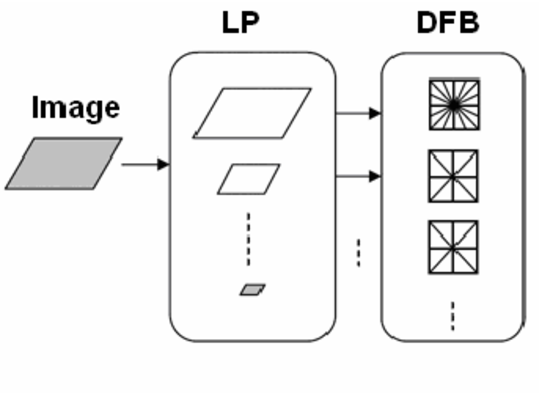
\includegraphics[width=0.7\textwidth]{fig/contourlet}
	\caption{\glsdesc{ct}}
	\label{fig:contourlet}
\end{figure}

\subsection{Definition}

The \gls{ct} is a directional transform, capable of capturing contours and fine details in images. The Figure \ref{fig:contourlet_2} illustrates the \gls{ct}, in which the input image consists of frequency components like \gls{ll}, \gls{lh}, \gls{hl} and \gls{hh}. 

\begin{figure}[H]
	\centering
	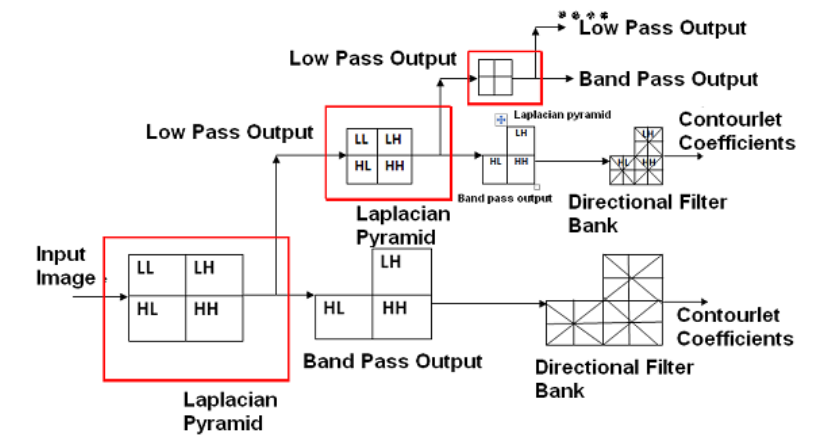
\includegraphics[width=0.7\textwidth]{fig/contourlet_2}
	\caption{Flowchart of \glsdesc{ct}}
	\label{fig:contourlet_2}
\end{figure}

The \gls{lp} at each level generates a Low pass output (LL) and a Band pass output (LH, HL, and HH). The Band pass output is then passed into \gls{dfb}, which
results in contourlet coefficients. The Low pass output is again passed through the \gls{lp} to obtain more coefficients and this is done till the fine details of the image are obtained. Figure \ref{fig:contourlet_mr} shows the decomposition of brain MR Image. 

\begin{figure}[H]
	\centering
	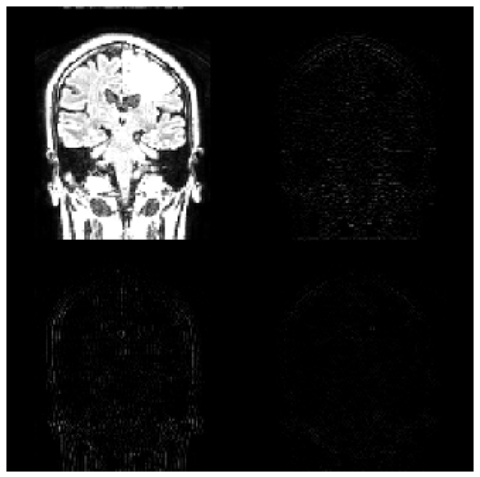
\includegraphics[width=0.45\textwidth]{fig/contourlet_mr}
	\caption{Contourlet decomposition of brain MR Image}
	\label{fig:contourlet_mr}
\end{figure}



